\documentclass{article}
\usepackage{tikz}

\usetikzlibrary{shapes,arrows,decorations.markings}

\tikzset{every node/.style={circle},
         strike through/.append style={
    decoration={markings, mark=at position 0.5 with {
    \draw[-] ++ (-5pt,-5pt) -- (5pt,5pt);}
  }, postaction={decorate}}
}

\tikzstyle{block} = [rectangle, draw, fill=blue!20,
    text width=5em, text centered, rounded corners, minimum height=4em]
\tikzstyle{line} = [draw, -latex']
\tikzstyle{xline} = [draw, strike out, -latex']

\begin{document}

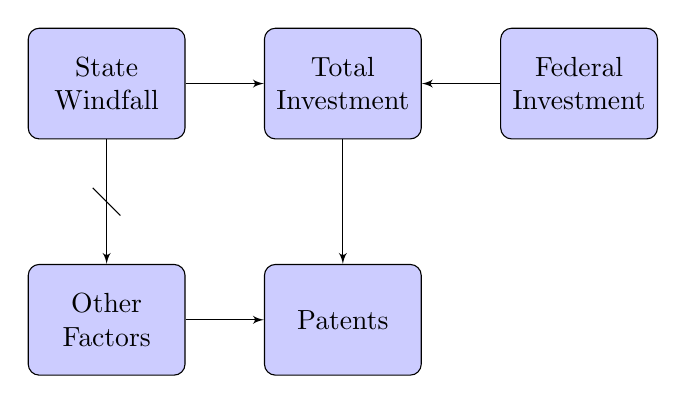
\begin{tikzpicture}[node distance = 3cm, auto]
    \node [block] (wind) {State Windfall};
    \node [block, right of=wind] (invtot) {Total Investment};
    \node [block, right of=invtot] (invfed) {Federal Investment};
    \node [block, below of=wind] (other) {Other Factors};
    \node [block, right of=other] (pats) {Patents};
    \path [line] (wind) edge (invtot);
    \path [line] (wind) edge [strike through] (other);
    \path [line] (other) edge (pats);
    \path [line] (invtot) edge (pats);
    \path [line] (invfed) edge (invtot);
\end{tikzpicture}

\end{document}
